\section{Evaluation Results with Baseline Comparison}

\begin{table*}[!ht]
\centering
\footnotesize
\begin{tabular}{c|cccc|c}
\toprule
&  \multicolumn{4}{c}{\textbf{Generative Models}}  \\
\cmidrule{2-6}
\textbf{Task} & \textbf{Mem2Seq*} & \textbf{Seq2Seq} & \textbf{Seq2Seq+Copy} & \textbf{Mem2Seq} & \textbf{ \sys\ }  \\
\midrule
T1 & 100 (100) & 100 (100) & 100 (100) & 100 (100) & 100 (100) \\
T2 & 100 (100) &  100 (100) &  100 (100) & 100 (100) & 100 (100) \\
T3 & 94.7 (62.1) & 74.8 (0) & 85.1 (19.0)& 74.9 (0) & \textbf{95.2 (63.8)}    \\
T4 & 100 (100) & 57.2 (0) & 100 (100) & 100 (100)  & 100 (100) \\
T5 & \textbf{97.9 (69.6)} & 97.2 (64.4) & 96 (49.1)  & 97.7(66.3) & 97.3 (65.6) \\
\midrule
T1-OOV & 94.0 (62.2) & 81.7 (0) & 92.5 (54.7)  & 94.0 (62.2) & \textbf{100 (100)}\\
T2-OOV & 86.5 (12.4)  & 78.9 (0) & 83.2 (0) & 86.5 (12.4) & \textbf{100 (100)}\\
T3-OOV & 90.3 (38.7) & 75.3 (0) & 82.9 (0) & 75.2 (0) &  \textbf{95.7 (66.6)}   \\
T4-OOV & 100 (100) & 57.0 (0) & 100 (100) & 100 (100) & 100 (100) \\
T5-OOV & 84.5 (2.3) & 67.4 (0) & 73.6 (0) & 75.6 (0) & \textbf{91.7 (18.5)}   \\
\bottomrule
\end{tabular}
\caption{Per-response and per-dialog accuracies (in brackets) on bAbI dialog tasks of \sys\ and other generative model baselines. We highlight the best accuracies achieved for each task.} 
\label{tab:Ababi}
\end{table*}

\begin{table*}[!ht]
\centering
\footnotesize
\begin{tabular}{c|ccc|c}
\toprule
& \multicolumn{3}{c|}{\textbf{Retrieval Models}} & \multicolumn{1}{c}{\textbf{Generative Models}}  \\
\cmidrule{2-5}
\textbf{Task} & \textbf{QRN} & \textbf{MN} &  \textbf{GMN} & \textbf{ \sys\ }  \\
\midrule
T1 & 99.9 (-) & 99.6 (99.6) & 100 (100) & 100 (100) \\
T2 & 99.5 (-) & 100 (100) & 100 (100)& 100 (100) \\
T3 & 74.8 (-) & 74.9 (2.0) & 74.9 (0)& \textbf{95.2 (63.8)}    \\
T4 & 57.2 (-) & 59.5 (3.0) & 57.2 (0)& \textbf{100 (100)} \\
T5 & \textbf{99.6 (-)} & 96.1 (49.4) & 96.3 (52.5) & 97.3 (65.6) \\
\midrule
T1-OOV & 83.1 (-) & 72.3 (0) & 82.4 (0) & \textbf{100 (100)}\\
T2-OOV & 78.9 (-) & 78.9 (0) & 78.9 (0) & \textbf{100 (100)}\\
T3-OOV & 75.2 (-) & 74.4 (0) & 75.3 (0) & \textbf{95.7 (66.6)}   \\
T4-OOV & 56.9 (-) & 57.6 (0) & 57.0 (0) & \textbf{100 (100)} \\
T5-OOV & 67.8 (-) & 65.5 (0) & 66.7 (0) & \textbf{91.7 (18.5)}   \\
\bottomrule
\end{tabular}
\caption{Per-response and per-dialog accuracies (in brackets) on bAbI dialog tasks of \sys\ and other retrieval model baselines}. 
\label{tab:babi}
\end{table*}

\begin{table}[!ht]
\centering
\footnotesize
 \begin{tabular}{l|cc|cc}
\toprule
& \multicolumn{2}{c|}{\textbf{CamRest}} & \multicolumn{2}{c}{\textbf{SMD}}  \\ \cmidrule{2-5}
& \textbf{BLEU} & \textbf{Ent. F1} & \textbf{BLEU} & \textbf{Ent. F1} \\
\midrule
Mem2Seq* & 12.7 & 39 & 12.6 & 33.4  \\
\midrule
Seq2Seq & 11.4 & 40.6 & 8.7 & 34.9  \\
%Seq2Seq+Attn & & & 9.3 & 19.9 \\
Seq2Seq+Copy & 4.7 & 32.2 & 3.23 & 16.9  \\
Mem2Seq & 12.7 & 39 & \textbf{10.3} & 31.8 \\ 
\midrule
\sys\ & \textbf{15.2} & \textbf{43.1} & 8.3 & \textbf{35.9} \\
\bottomrule
\end{tabular}
\caption{Performance of \sys\ and baselines on the CamRest and SMD datasets}
\label{tab:Asmd}
\end{table}

\begin{table}[!ht]
\centering
\footnotesize
 \begin{tabular}{l|cc|cc}
\toprule
& \multicolumn{2}{c|}{\textbf{CamRest}} & \multicolumn{2}{c}{\textbf{SMD}}  \\ \cmidrule{2-5}
& \textbf{Info} & \textbf{Grammar} & \textbf{Info} & \textbf{Grammar} \\
\midrule
Seq2Seq & 46 & 2.24 & 35 &  2.38 \\
Seq2Seq+Copy & 27 & 1.1 & 21 &  1.04 \\
Mem2Seq & 51 & 2.2 & \textbf{38} &  2.0 \\
\midrule
\sys\ & \textbf{77} & \textbf{2.28} & 36 &  \textbf{2.5} \\

\bottomrule
\end{tabular}
\caption{AMT Evaluations on CamRest and SMD} 
\label{tab:Aamt_perf}
\end{table}

\begin{table}[!ht]
\centering
\footnotesize
 \begin{tabular}{l|cc|cc}
\toprule
& \multicolumn{2}{c|}{\textbf{CamRest}} & \multicolumn{2}{c}{\textbf{SMD}}  \\ \cmidrule{2-5}
& \textbf{Info} & \textbf{Grammar} & \textbf{Info} & \textbf{Grammar} \\
\midrule
Seq2Seq & 26 & 2.28 & 22 & \textbf{2.44} \\
Seq2Seq+Copy & 22 & 1.22 & 16 & 1.04 \\
Mem2Seq & 35 & 2.06 & 26 & 1.9 \\
\midrule
\sys\ & \textbf{80} & \textbf{2.44} & \textbf{51} &  2.28 \\

\bottomrule
\end{tabular}
\caption{AMT Evaluations on CamRest and SMD (50\% unseen) KA datasets} 
\label{tab:Aamt_dis}
\end{table}

\begin{table}[!ht]
\centering
\footnotesize
% \vspace{2mm}
\begin{tabular}{l|c|c|c}
\toprule
   & \textbf{bAbI Dialog} & \textbf{bAbI Dialog (OOV)}  & \textbf{CamRest} \\ \cmidrule{2-4}
    & Avg. Response Acc.  & Avg. Response Acc. & Ent. F1       \\ \midrule
\sys\ w/o {\sc BoSs} Memory & 85.54 & 77.14 & 29          \\
\sys\ w/o $\mathcal{L}_{d}$          & 97.2 & 84.3 & 40.1          \\
\sys\  w/o DLD     & 97.74 & 86.52 & 40.45         \\ \midrule
\sys\                 & 98.5    & 97.48 & 43.1    
\\ \bottomrule
\end{tabular}
\caption{Ablation study: impact of each model element on \sys\ }
\label{tab:Aablation}
\end{table}

\begin{table}[!ht]
\centering
\footnotesize
\begin{tabular}{l|ccccc|ccccc|cc}
\toprule
   & \multicolumn{5}{c|}{\textbf{bAbI Dialog Tasks}} & \multicolumn{5}{c|}{\textbf{bAbI Dialog Tasks (OOV)}}  & \multicolumn{2}{c}{\textbf{CamRest}} \\ \cmidrule{2-6} \cmidrule{7-11} \cmidrule{12-13}
    & T1  & T2  & T3   & T4   & T5   & T1 & T2 & T3 & T4 & T5 & BLEU        & Ent. F1       \\ \midrule
1-Hop  & 100 & 100 & 92.3 & 100 & 90.5 & 100 & 100 & 91.4 & 100 & 89 & 10.5 & 36.9 \\
Multi-Hop  & 100 & 100 & 95.2 & 100  & 97.3 & 100    & 100    & 95.7   & 100    & 91.7   & 15.2        & 43.1    
\\ \bottomrule
\end{tabular}
\caption{Ablation study: impact of hops in \sys\ encoder }
\label{tab:Aablationhop}
\end{table}

\clearpage

\section{Dataset Preprocessing and Faults}
\label{sec:preprocess}
\subsection{Mem2Seq Preprocessing}
\label{sec:prep_mem}

\begin{figure*}[ht]
\centering
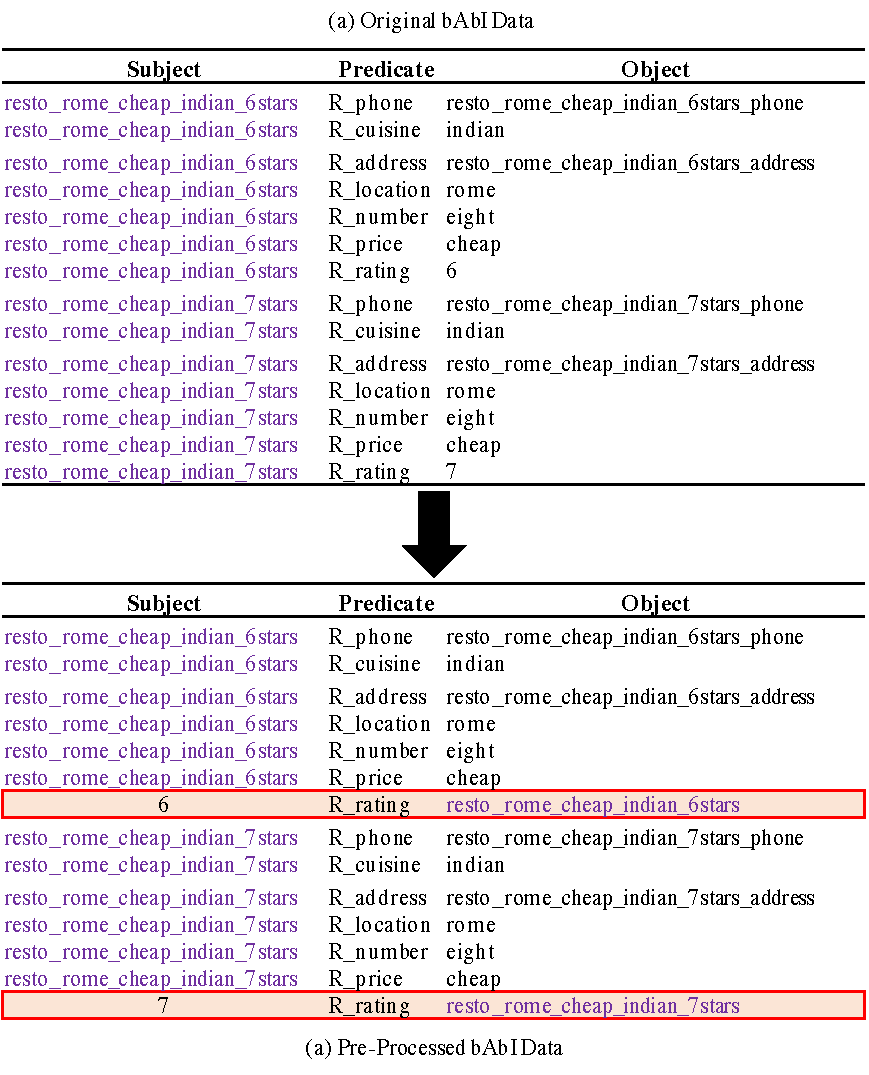
\includegraphics[width=0.8\textwidth]{assets/babi-preprocess.pdf}
\caption{Pre-processing of bAbI dialog data used in Mem2Seq paper}
\label{fig:prebabi}
\end{figure*}

\begin{figure*}[ht]
\centering
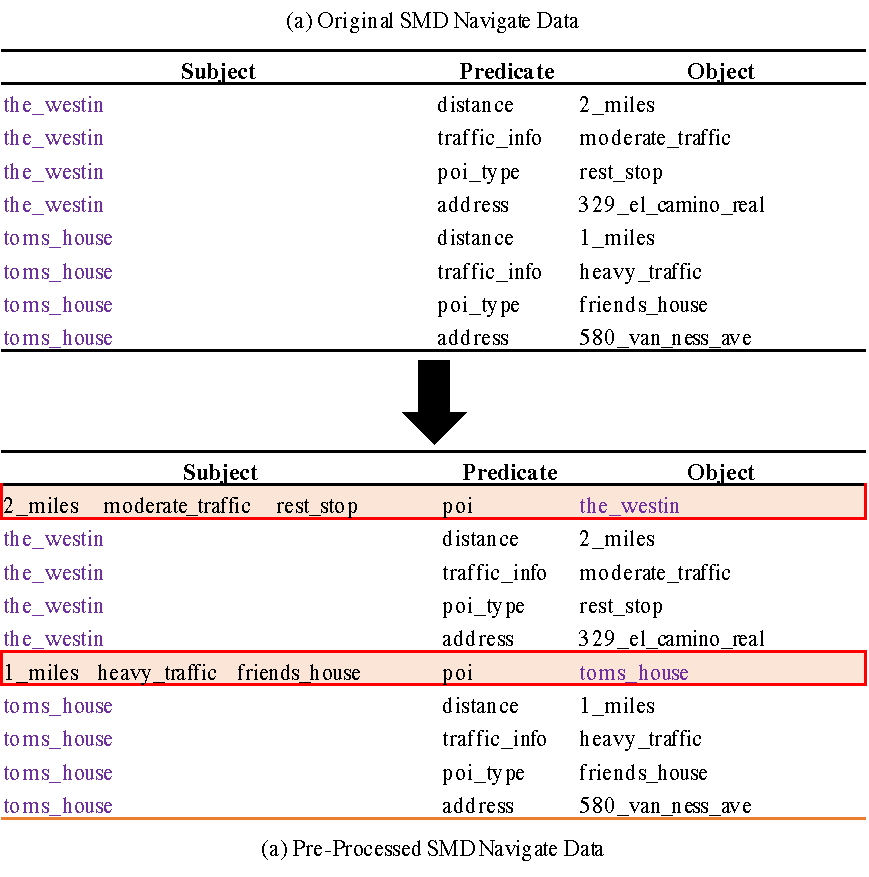
\includegraphics[width=0.8\textwidth]{assets/smd-preprocess.pdf}
\caption{Pre-processing of SMD Navigate data used in Mem2Seq paper}
\label{fig:presmd}
\end{figure*}

Mem2Seq paper used the following pre-processing on the data:
\begin{enumerate}
    \item The subject (restaurant name) and object (rating) positions of the rating KB tuples in bAbI dialogs are flipped, while the order remains the same for other tuples remains the same. This pre-processing is illustrated in Figure \ref{fig:prebabi}
    \item an extra fact was added to the navigation tasks in In-Car Assistant with all the properties (such as distance, address) combined together  as the subject and \textit{poi} as the object. This pre-processing is illustrated in Figure \ref{fig:presmd}
\end{enumerate}
The pre-processing has major impact on the performance of  Mem2Seq, as it can only copy objects of a KB tuple, while the subject and relation can never be copied.

\subsection{bAbI Dataset Faults}
\label{sec:fault}
The KB entities present in validation and non-OOV test sets for task 3 and 4 do not overlap with those in the train set. This effectively means that non-OOV and OOV test conditions are the same for tasks 3 and 4. This explains the low performance of baseline models on task 3 and 4 non-OOV test sets.

\section{Example Predictions of \sys\ and Baselines}
\label{sec:examples}
Examples from SMD is shown in Table \ref{tab:smd0} respectively. Examples from KA test set with percentage of unseen entites set to 50 from CamRest and SMD are shown in Table \ref{tab:cam50} and Table \ref{tab:smd50} respectively. Examples from KA test set with percentage of unseen entites set to 100 from bAbI dialog Task 1 is shown in Table \ref{tab:t1_100}.

\begin{table*}
\centering
\small
\begin{tabular}{c|l}

\toprule
% \multicolumn{2}{c}{\textbf{KB (restaurant|cuisine|address|phone|postcode)}} \\
% \multicolumn{2}{c}{\textit{prezzo}|\textit{ethiopian}|\textit{22\_seetharam\_nagar}|\textit{01799\_521260}|\textit{cb30ad}}\\
% \midrule
\midrule
\textbf{usr-1} &good morning \\
\textbf{sys-1} & hello what can i help you with today \\
\textbf{usr-2} & can you book a table with \textit{korean} cuisine for \textit{five} in \textit{beijing} \\
\textbf{sys-2} & i ' m on it . which price range are looking for ? \\
\textbf{usr-3} & i am looking for a \textit{overpriced} restaurant \\
\midrule
\textbf{Gold} & api\_call \textit{korean beijing five overpriced}
 \\
\midrule
\midrule
\specialcell[t]{\textbf{Seq2Seq+Copy}} & api\_call \textit{korean beijing five overpriced}
 \\
\midrule
\textbf{Seq2Seq} & api\_call \textit{french london four moderate} \\

\midrule
\textbf{Mem2Seq} & api\_call \textit{overpriced korean korean overpriced}
 \\
\midrule
\textbf{\sys\ } & api\_call \textit{korean beijing five overpriced} \\
\bottomrule
\end{tabular}
\caption{Example from bAbI dialog Task 1 with 100\% OOV.}
\label{tab:t1_100}
\end{table*}
\begin{table*}
\centering
\small
\begin{tabular}{c||p{13cm}}
\toprule
\multicolumn{2}{c}{\textbf{KB (restaurant|cuisine|address|phone|postcode)}} \\
\multicolumn{2}{c}{\textit{prezzo}|\textit{ethiopian}|\textit{22\_atlantis\_road}|\textit{01799\_521260}|\textit{cb30ad}}\\
\midrule
\midrule
\textbf{usr-1} &i want a \textit{moderately\_expensive ethiopian} restaurant in the \textit{south} side of town \\
\textbf{sys-1} & i ' m sorry . i can not find a \textit{moderately\_expensive ethiopian} restaurant in the \textit{south} side of town \\
\textbf{usr-2} & i would like to find a \textit{moderately} priced restaurant in the \textit{west} part of town \\
\textbf{sys-2} & \textit{prezzo} is a moderately priced \textit{ethiopian} restaurant in the \textit{west} part of town . there is also \textit{indian} and \textit{british} food available in that area and price range . would you like more info ? \\
\textbf{usr-3} & yes can i get thier address and postcode ? \\
\midrule
\textbf{Gold} & of course , \textit{prezzo} ' s address is \textit{22\_atlantis\_road} and postcode is \textit{cb30ad}
 \\
\midrule
\midrule
\specialcell[t]{\textbf{Seq2Seq+Copy}} & postcode a is is \textit{01223350688} UNK there get i for for today
 \\
\midrule
\textbf{Seq2Seq} & the address is \textit{83\_regent\_street} and their postcode is \textit{cb58aq} \\

\midrule
\textbf{Mem2Seq} & the phone address is \textit{cb21uj}
 \\
\midrule
\textbf{\sys\ } & the address is \textit{22\_atlantis\_road at 22\_atlantis\_road} the postcode is \textit{cb30ad} is there anything else i can help you with \\
\bottomrule
\end{tabular}
\caption{Example from Camrest with 50\% OOV. The OOV entities present in the dialog are \{\textit{ethiopian}, \textit{22\_atlantis\_road}\}}
\label{tab:cam50}
\end{table*}
\begin{table*}
\centering
\small
\begin{tabular}{c|p{13cm}}

\toprule
%\textbf{kb} & \textit{da\_vinci\_pizzeria}\\
% & \textit{r_phone|01223\_351707} \\
% & \textit{r_adddress|20\_milton\_road\_chesterton} \\
% & \textit{r_food|italian} \\
\multicolumn{2}{c}{\textbf{KB (location|distance|traffic info|address)}} \\
\multicolumn{2}{c}{\textit{teavana}|\textit{4\_miles}|\textit{no\_traffic}|\textit{145\_amherst\_st}}\\
\multicolumn{2}{c}{\textit{cafe\_venetia}|\textit{5\_miles}|\textit{moderate\_traffic}|\textit{269\_alger\_dr}}\\
\multicolumn{2}{c}{\textit{town\_and\_country}|\textit{3\_miles}|\textit{moderate\_traffic}|\textit{383\_university\_ave}}\\
\midrule
\midrule
\textbf{usr-1} & where can i get tea ? \\
\textbf{sys-1} & there is 2 tea shops near you \textit{teavana} is \textit{4\_miles} away and \textit{cafe\_venetia} is \textit{5\_miles} away which one do you want ? \\
\textbf{usr-2} & which one is the quickest is there any traffic ? \\
\midrule
\textbf{Gold} & \textit{teavana} is the fastest journey because there is \textit{no\_traffic} on the way there . \textit{cafe\_venetia} has \textit{moderate\_traffic} should we go to \textit{teavana}
 \\
\midrule
\midrule
\textbf{Seq2Seq+Copy} & there is
 \\
\midrule
\textbf{Seq2Seq} & there is \textit{moderate\_traffic} on the way to \textit{palo\_alto\_medical\_foundation} \\

\midrule
\textbf{Mem2Seq} & there is \textit{moderate\_traffic} on our way
 \\
\midrule
\textbf{\sys\ } & \textit{teavana} there is a \textit{moderate\_traffic} nearby but i might find another route to t\textit{own\_and\_country} \textit{town\_and\_country} address is \textit{383\_university\_ave} i sent it on your screen \\
\bottomrule
\end{tabular}
\caption{Example from SMD}
\label{tab:smd0}
\end{table*}

\begin{table*}
\centering
\small
\begin{tabular}{c|p{13cm}}

\toprule
\multicolumn{2}{c}{\textbf{KB (location|day|weather)}} \\
\multicolumn{2}{c}{\textit{mountain\_view}|\textit{sunday}|\textit{foggy}}\\
\multicolumn{2}{c}{\textit{mountain\_view}|\textit{monday}|\textit{overcast}}\\
\multicolumn{2}{c}{\textit{pittsburgh}|\textit{sunday}|\textit{overcast}}\\
\multicolumn{2}{c}{\textit{pittsburgh}|\textit{monday}|\textit{warm}}\\
\multicolumn{2}{c}{\textit{downtown\_chicago}|\textit{sunday}|\textit{foggy}}\\
\multicolumn{2}{c}{\textit{downtown\_chicago}|\textit{monday}|\textit{warm}}\\
\midrule
\multicolumn{2}{c}{\textit{today}|\textit{monday}}\\
\midrule
\midrule
\textbf{usr-1} &is the weather \textit{cloudy} right now ? \\
\textbf{sys-1} & what city do you want the weather for ? \\
\textbf{usr-2} & \textit{pittsburgh} \\
\midrule
\textbf{Gold} & there are no clouds in \textit{pittsburgh} right now
 \\
\midrule
\midrule
\textbf{Seq2Seq+Copy} & which is no
 \\
\midrule
\textbf{Seq2Seq} & it is currently raining in \textit{san\_francisco} right now \\

\midrule
\textbf{Mem2Seq} & it will not be cloudy in in
 \\
\midrule
\textbf{\sys\ } & it will be \textit{cloudy} on \textit{sunday} in \textit{pittsburgh} \\
\bottomrule 
\end{tabular}
\caption{Example from SMD with 50\% OOV. The OOV entity present in the dialog is \{\textit{pittsburgh}\}}
\label{tab:smd50}
\end{table*}
